\documentclass[a4paper, 12pt]{report}
\usepackage{graphicx}
\usepackage{amsmath, amsthm, amssymb}
\usepackage{enumerate}
\usepackage{enumitem}
\usepackage{array}
\usepackage{tabularx}
\usepackage{hyperref}
\usepackage{caption}
\usepackage[normalem]{ulem}
\usepackage{pdfpages}
\usepackage[toc,page]{appendix}
\usepackage{float}

\usepackage[chapter,newfloat]{minted}
\SetupFloatingEnvironment{listing}{name=Program}
\SetupFloatingEnvironment{listing}{listname=List of Programs}

%%% blank footnote
\newcommand\blfootnote[1]{
	\begingroup
	\renewcommand\thefootnote{}\footnote{#1}
	\addtocounter{footnote}{-1}
	\endgroup
}
%%%

%%% prevent hyphenation
\tolerance=1
\emergencystretch=\maxdimen
\hyphenpenalty=10000
\hbadness=10000
%%%

%%% make inline math look like display style math
\everymath{\displaystyle}

%%% minimize
\DeclareMathOperator*{\minimize}{minimize}
%%%

% Theorem environments
\newtheorem{theorem}{Theorem}
\newtheorem{corollary}[theorem]{Corollary}
\newtheorem{lemma}[theorem]{Lemma}
\newtheorem{proposition}[theorem]{Proposition}
\newtheorem{conjecture}[theorem]{Conjecture}
\newtheorem{observation}[theorem]{Observation}

\theoremstyle{definition}
\newtheorem{definition}[theorem]{Definition}
\newtheorem{question}[theorem]{Question}

\theoremstyle{remark}
\newtheorem*{remark}{Remark}

%%%
\def\N{\mathbb{N}}
\def\Z{\mathbb{Z}}
\def\Q{\mathbb{Q}}
\def\R{\mathbb{R}}
\def\F{\mathbb{F}}

\def\tends{\rightarrow}
\def\into{\rightarrow}
\def\half{\frac{1}{2}}
\def\quarter{\frac{1}{4}}

\newcommand{\set}[1]{\left\{ #1 \right\}}
\newcommand{\norm}[1]{\left\Vert #1 \right\Vert}
\newcommand{\card}[1]{\left\vert #1 \right\vert}
\newcommand{\ceil}[1]{\left\lceil #1 \right\rceil}
\newcommand{\floor}[1]{\left\lfloor #1 \right\rfloor}

\DeclareMathOperator{\dia}{dia}
%%%

\title{Notes\\
\large Introduction to Computer Science (CS50) on EdX}
\author{Sparsh Jain}
\date{\today}

\begin{document}

\maketitle
\tableofcontents
% \listoffigures
% \listoftables
\listoflistings

% \include{chapters/introduction}
\chapter{Computational Thinking, Scratch}
\section{Binary Number System}
\section{Algorithms}
\section{Time Complexity}
\section{Pseudocode}
\section{Scratch}

\blfootnote{This was only an introductory lecture.
    Click \href{https://www.youtube.com/watch?v=jjqgP9dpD1k}{here} for more details.}
\chapter{C}
\section{Hello World}
\begin{listing}[ht!]
	\inputminted[linenos]{c}{codes/helloWorld.c}
	\caption{Hello World in C}
\end{listing}

\begin{remark}
	Need to compile using a compiler like \mintinline{bash}{clang} or
	\mintinline{bash}{gcc}.
\end{remark}

\section{Input}
\begin{listing}[ht!]
	\inputminted[linenos]{c}{codes/helloUser.c}
	\caption{Hello User in C}
\end{listing}

\begin{remark}
	In case of errors in compiling, start by trying to \emph{fix} the first one, and so on.
\end{remark}

\begin{remark}
	Use \mintinline{bash}{-lcs50} to link \mintinline{c}{cs50.h} header.
\end{remark}

\begin{remark}
	Use \mintinline{bash}{make} to ease your life compiling!
\end{remark}

\clearpage
\section{Initialization}
\begin{minted}{c}
	int counter = 0;
\end{minted}

\section{Increment}
\begin{minted}{c}
	counter = counter + 1;
	counter += 1;
	counter++; // Syntactic Sugar
\end{minted}

\section{Conditionals}
\begin{minted}{c}
	if (x < y)
	{
		printf("x is less than y!\n");
	}
	else if (x > y)
	{
		printf("x is greater than y!\n");
	}
	else // if (x == y)
	{
		printf("x is equal to y!\n");
	}
\end{minted}

\section{Loops}
\subsection{While Loop}
\subsubsection{Infinite Loop}
\begin{minted}{c}
	while(true)
	{

	}
\end{minted}

\subsubsection{Repeat}
\begin{minted}{c}
	int i = 0;
	while(i < 50)
	{
		printf("Hello World!\n");
		i = i+1;
	}
\end{minted}

\subsection{For Loop}
\begin{minted}{c}
	for(int i = 0; i < 50; i += 1)
	{
		printf("Hello World!\n");
	}
\end{minted}

\section{Additional Info}
\subsection{Datatypes}
Some of these (like \mintinline{c}{string}) are implemented in \mintinline{c}{cs50.h} library.
\begin{itemize}
	\item \mintinline{c}{bool}
	\item \mintinline{c}{char}
	\item \mintinline{c}{double}
	\item \mintinline{c}{float}
	\item \mintinline{c}{int}
	\item \mintinline{c}{long}
	\item \mintinline{c}{string}
	\item \dots
\end{itemize}

\subsection{Functions}
They are implemented in \mintinline{c}{cs50.h} library.
\begin{itemize}
	\item \mintinline{c}{get_char}
	\item \mintinline{c}{get_float}
	\item \mintinline{c}{get_double}
	\item \mintinline{c}{get_int}
	\item \mintinline{c}{get_long}
	\item \mintinline{c}{get_string}
	\item \dots
\end{itemize}

\subsection{Placeholders}
\begin{itemize}
	\item \mintinline{c}{%c} for \mintinline{c}{char}
	\item \mintinline{c}{%f} for \mintinline{c}{float}
	\item \mintinline{c}{%i} for \mintinline{c}{int}
	\item \mintinline{c}{%li} for \mintinline{c}{long}
	\item \mintinline{c}
\end{itemize}


\section{Examples}
\subsection{Arithmetic}
\begin{listing}[ht!]
	\inputminted[linenos]{c}{codes/int.c}
	\caption{int.c}
\end{listing}

\begin{listing}[ht!]
	\inputminted[linenos]{c}{codes/float.c}
	\caption{float.c}
\end{listing}

\begin{listing}[ht!]
	\inputminted[linenos]{c}{codes/parity.c}
	\caption{parity.c}
\end{listing}

\clearpage
\subsection{Conditional}
\begin{listing}[ht!]
	\inputminted[linenos]{c}{codes/conditions.c}
	\caption{conditions.c}
\end{listing}

\clearpage
\subsection{Logical}
\begin{listing}[ht!]
	\inputminted[linenos]{c}{codes/agree.c}
	\caption{agree.c}
\end{listing}

\clearpage
\subsection{Loop}
\begin{listing}[ht!]
	\inputminted[linenos]{c}{codes/src1/cough0.c}
	\caption{cough0.c}
\end{listing}

\begin{listing}[ht!]
	\inputminted[linenos]{c}{codes/src1/cough1.c}
	\caption{cough1.c}
\end{listing}

\clearpage
\subsection{Function}
\begin{listing}[ht!]
	\inputminted[linenos]{c}{codes/src1/cough2.c}
	\caption{cough2.c}
\end{listing}

\begin{listing}[ht!]
	\inputminted[linenos]{c}{codes/src1/cough3.c}
	\caption{cough3.c}
\end{listing}

\begin{listing}[ht!]
	\inputminted[linenos]{c}{codes/src1/positive.c}
	\caption{positive.c}
\end{listing}

\begin{listing}[ht!]
	\inputminted[linenos]{c}{codes/src1/mario0.c}
	\caption{mario0.c}
\end{listing}

\begin{listing}[ht!]
	\inputminted[linenos]{c}{codes/src1/mario2.c}
	\caption{mario2.c}
\end{listing}

\begin{listing}[ht!]
	\inputminted[linenos]{c}{codes/src1/mario8.c}
	\caption{mario8.c}
\end{listing}

\clearpage
\section{Limitations}
\begin{listing}[ht!]
	\inputminted[linenos]{c}{codes/src1/floats.c}
	\caption{floats.c}
\end{listing}

\begin{listing}[ht!]
	\inputminted[linenos]{c}{codes/src1/overflow.c}
	\caption{overflow.c}
\end{listing}

\blfootnote{Click \href{pdfs/src1.pdf}{here} for more examples.}

% \clearpage
% \section{Source Code}
% Find some pre-compiled examples below
% 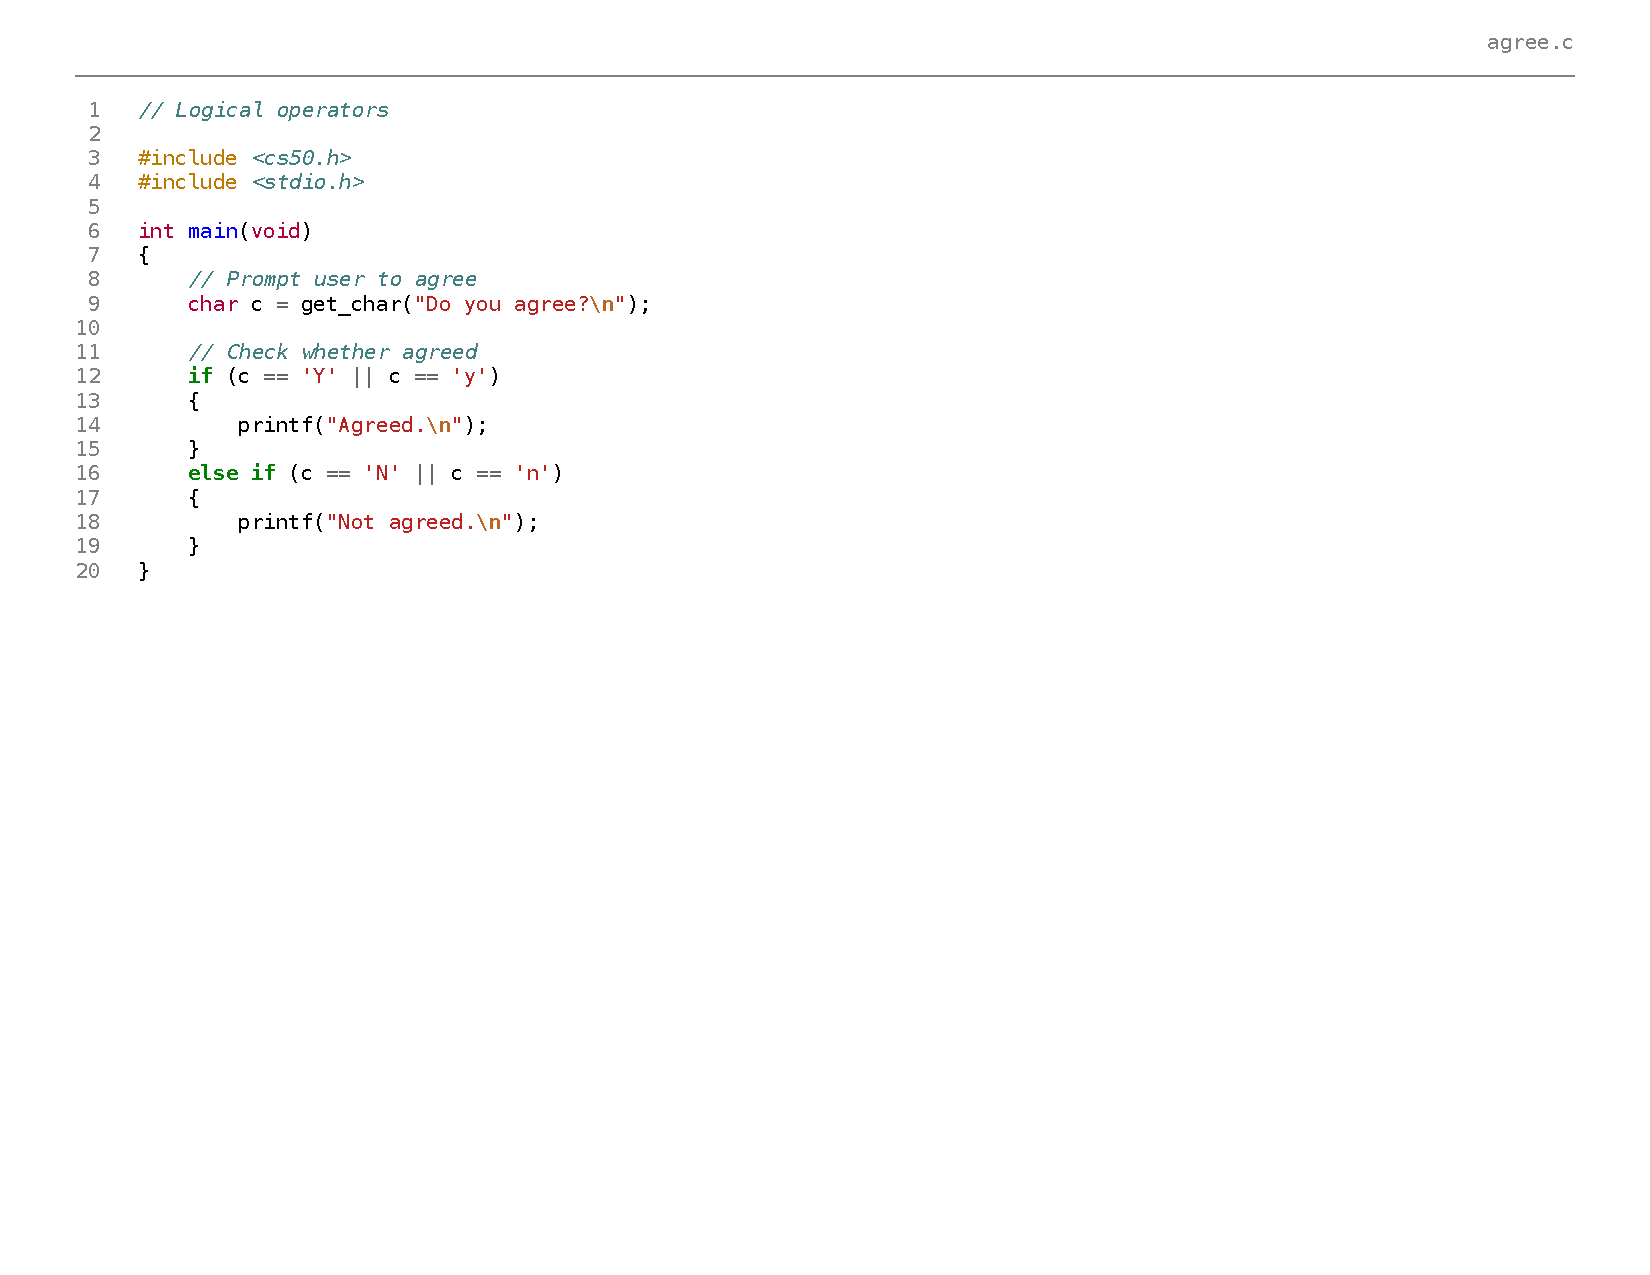
\includepdf[pages=-]{pdfs/src1.pdf}
\chapter{Arrays}
\section{Compiling}
\subsection{Preprocessing}
Expansion/Inclusion of header files, macros, etc.

\subsection{Compiling}
C code $\to$ Assembly code.

\subsection{Assembling}
Assembly code $\to$ Machine code.

\subsection{Linking}
Linking all relevent files.

\section{Debugging}
\begin{itemize}
    \item Can use \mintinline{bash}{help50} to understand error msgs in this course.
    \item Can use (poor man's) \mintinline{c}{printf}.
    \item Can use \mintinline{bash}{debug50} for proper debugging (in this course).
\end{itemize}

\begin{remark}
    Use \mintinline{bash}{style50} for styling your code.
\end{remark}

\section{Casting}
\begin{code}[ht!]
    \inputminted[linenos]{c}{codes/src2/hi.c}
    \caption{casting}
\end{code}

\section{Array}
Follow through the following examples:
\begin{code}[htbp!]
    \inputminted[linenos]{c}{codes/src2/scores0.c}
    \caption{scores0.c}
\end{code}

\begin{code}[htbp!]
    \inputminted[linenos]{c}{codes/src2/scores1.c}
    \caption{scores1.c}
\end{code}

\begin{code}[htbp!]
    \inputminted[linenos]{c}{codes/src2/scores2.c}
    \caption{scores2.c}
\end{code}

\begin{code}[htbp!]
    \inputminted[linenos]{c}{codes/src2/scores3.c}
    \caption{scores3.c}
\end{code}

% \clearpage
\section{String}
\mintinline{c}{string} is just (or a little more) than an array of \mintinline{c}{chars}.

\begin{code}[!htbp]
    \inputminted[linenos]{c}{codes/src2/names.c}
    \caption{names.c}
\end{code}

\begin{code}[!htbp]
    \inputminted[linenos]{c}{codes/src2/string0.c}
    \caption{string0.c}
\end{code}

\begin{code}[!htbp]
    \inputminted[linenos]{c}{codes/src2/string1.c}
    \caption{string1.c}
\end{code}

\begin{code}[!htbp]
    \inputminted[linenos]{c}{codes/src2/string2.c}
    \caption{string2.c}
\end{code}

\begin{code}[!htbp]
    \inputminted[linenos]{c}{codes/src2/uppercase0.c}
    \caption{uppercase0.c}
\end{code}

\begin{code}[!htbp]
    \inputminted[linenos]{c}{codes/src2/uppercase1.c}
    \caption{uppercase1.c}
\end{code}

\clearpage
\section{Command Line Arguments}
\begin{code}[!htbp]
    \inputminted[linenos]{c}{codes/src2/argv.c}
    \caption{argv.c}
\end{code}

\begin{code}[!htbp]
    \inputminted[linenos]{c}{codes/src2/argv2.c}
    \caption{argv2.c}
\end{code}

\begin{code}[!htbp]
    \inputminted[linenos]{c}{codes/src2/exit.c}
    \caption{exit.c}
\end{code}

%%% chapter endnote
% \blfootnote{Check \href{lecture_pdf/Lecture1.pdf}{Lecture1.pdf} for more details.}

% \begin{appendices}
% \end{appendices}

\end{document}